\chapter{The Dot Product}
% Reference for diagrams:https://www.mathsisfun.com/algebra/vectors-dot-product.html

If you have two vectors $\textbf{u} = [u_1, u_2, \dots, u_n]$ and $\textbf{v} 
= [v_1, v_2,\dots, v_n]$, we define the \newterm{dot product} $\textbf{u} 
\cdot \textbf{v}$ as 
\begin{equation*}
     \textbf{u} \cdot \textbf{v} = (u_1 \times v_1) + (u_2 \times v_2) + \dots 
     + (u_n \times v_n)
\end{equation*} 
The output of the dot product is a \emph{scalar} quantity.


For example, 
\begin{equation*}
    [2,4, -3] \cdot [5, -1, 1] = 2 \times 5 + 4 \times -1 + -3 \times 1 = 3
\end{equation*}\index{dot product}

This may not seem like a very powerful idea, but dot products are 
\emph{incredibly} useful. The enormous GPUs (Graphics Processing Units) that 
let video games render scenes so quickly? They primarily function by computing 
huge numbers of dot products at mind-boggling speeds. 

\begin{Exercise}[title={Basic dot products}, label=dot_products]
    Compute the dot product of each pair of vectors:
    \begin{itemize}
        \item $[1, 2, 3]$, $[4, 5, -6]$
        \item $[\pi, 2\pi]$, $[2, -1]$
        \item $[0,0,0,0]$, $[10,10,10,10]$
    \end{itemize}
\end{Exercise}
\begin{Answer}[ref=dot_products]
        \begin{itemize}
            \item $[1, 2, 3] \cdot [4, 5, -6] = 4 + 10 - 18 = -4$
            \item $[\pi, 2\pi] \cdot [2, -1] = 2\pi - 2\pi = 0$
            \item $[0,0,0,0] \cdot [10,10,10,10] = 0 + 0 + 0 + 0 = 0$ 
        \end{itemize}
\end{Answer}

\section{Properties of the dot product}

Sometimes we need an easy way to say ``The vector of appropriate length is 
filled with zeros.'' We use the notation $\vec{0}$ to represent this. Then, 
for any vector $\textbf{v}$, this is true:

$$\textbf{v} \cdot \vec{0} = 0$$

The dot product is commutative:

$$\textbf{v} \cdot \textbf{u} = \textbf{u} \cdot \textbf{v}$$

The dot product of a vector with itself is its magnitude squared:

$$ \textbf{v} \cdot \textbf{v} = |\textbf{v}|^2 $$

If you have a scalar $a$, then:

    $$(\textbf{v}) \cdot (a \textbf{u}) = a (\textbf{v} \cdot \textbf{u})$$

So, if $\textbf{v}$ and $\textbf{w}$ are vectors that go in the same direction,

    $$\textbf{v} \cdot \textbf{w} = |\textbf{v}| |\textbf{w}|$$

If $\textbf{v}$ and $\textbf{w}$ are vectors that go in opposite directions,

    $$\textbf{v} \cdot \textbf{w} = -|\textbf{v}| |\textbf{w}|$$
    
If $\textbf{v}$ and $\textbf{w}$ are vectors that are perpendicular to each 
other, their dot product is zero:

  $$ \textbf{v} \cdot \textbf{w} = 0 $$

\section{Cosines and dot products}

Furthermore, dot products' interaction with cosine makes them even more useful 
is what makes them so useful: 
If you have two vectors $\textbf{v}$ and $\textbf{u}$,

$$\textbf{v} \cdot \textbf{u} = |\textbf{v}| |\textbf{u}| \cos \theta$$

where $\theta$ is the angle between them.

So, for example, if two vectors $\textbf{v}$ and $\textbf{u}$ are 
perpendicular, the angle between them is $\pi/2$. The cosine of $\pi/2$ is 0. 
The dot product of any two perpendicular vectors is always 0. In fact, if the 
dot product of two non-zero vectors is 0, the vectors \textit{must be} 
perpendicular (see figure \ref{fig:perpendicular} for an example of 
perpendicular 2-dimensional vectors). 

\begin{figure}[htbp]
    \centering
    \begin{tikzpicture}
        \begin{axis}[xmin = -2, xmax = 5, ymin = 0, ymax = 5, 
        axis lines = center]
            \draw[blue, thick, -latex] (0, 0) -- (-1, 4) 
            node[above, black, font = \scriptsize] {$\left[ -1, 4 \right]$};
            \draw[blue, thick, -latex] (0, 0) -- (4, 1) 
            node[above, black, font = \scriptsize] {$\left[ 4, 1 \right]$};
        \end{axis}
    \end{tikzpicture}
    \caption{The dot product of any two perpendicular vectors is zero.}
    \label{fig:perpendicular}
\end{figure}
% cosine is not introduced before here
If you have two non-zero vectors $\textbf{v}$ and $\textbf{u}$, you can always 
compute the angle between them:\index{vectors!angle between}

$$\theta = \arccos{ \left( \frac{\textbf{v} \cdot \textbf{u}}{|\textbf{v}| 
|\textbf{u}|} \right)}$$

Arccos is short for arccosine, or $\cos^-1$, and it is a function that is the 
inverse of cosine. Cosine takes an angle and gives back the scaled 
$x$-component of the angle. Arccosine takes the $x$-component of an angle and 
returns an angle with that $x$-component. However, there is a limit to what 
arccos can return. Let's look at cosine and its inverse, arccos (see figures 
\ref{fig:cosine} and \ref{fig:arccos}). 

\begin{figure}[htbp]
    \centering
        \begin{tikzpicture}
            \begin{axis}[xmin = -0.5, xmax = 7, ymin = -1.25, ymax = 1.25, 
            axis lines = center, xlabel = $x$, ylabel = $y$]
                \addplot[blue, thick, samples = 150, domain = -0.5:7] 
                {cos(deg(x))};
            \end{axis}
        \end{tikzpicture}
        \caption{Cosine is a function: there is exactly one output for every 
        input.}
    \label{fig:cosine}
\end{figure}

\begin{figure}[htbp]
    \centering
    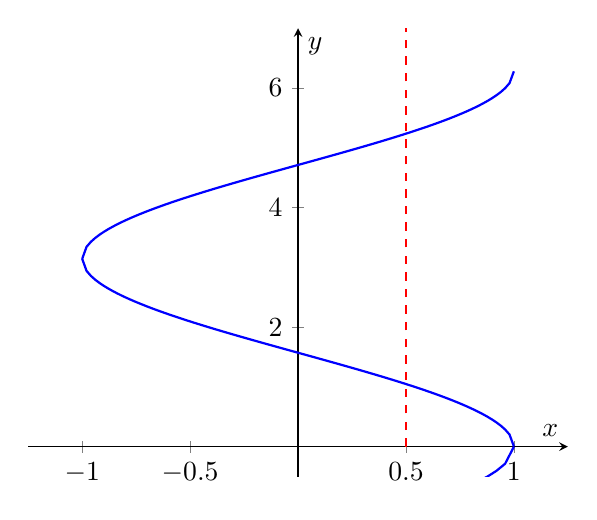
\begin{tikzpicture}
            \begin{axis}[xmin = -1.25, xmax = 1.25, ymin = -0.5, ymax = 7, 
            axis lines = center, xlabel = $x$, ylabel = $y$]
                \addplot[domain = -1:1, samples = 50, blue, thick]
                {-1*rad(acos(x))};
                \addplot[domain = -1:1, samples = 100, blue, thick]
                {rad(acos(x))};
                \addplot[domain = -1:1, samples = 100, blue, thick]
                {-1*rad(acos(x)) + 6.28319};
                \draw[red, thin, dashed] (0.5, 0) -- (0.5, 7);
            \end{axis}
        \end{tikzpicture}
    \caption{Arccos is not a function: there are many angles with the same 
    $x$-component. Notice that one input value has many output values (see the 
    red dashed line).}
    \label{fig:arccos}
\end{figure}

When you use a calculator to evaluate arccos, the calculator automatically 
restricts the results to between $0$ and $\pi$. Let's look at an example of 
using the dot product to determine the angle between two vectors:

\textbf{Example}: What is the angle between $\textbf{u} = \left[ \sqrt{3}, 1 
\right]$ and $\textbf{v} = \left[ 0, -1 \right]$?

\textbf{Solution}: We know that $\textbf{u} \cdot \textbf{v} = \left| 
\textbf{u} \right| \left| \textbf{v} \right| \cos{\theta}$. Therefore, we also 
know that:
$$\cos{\theta} = \frac{\textbf{u} \cdot \textbf{v}}{\left| \textbf{u} \right| 
\left| \textbf{v} \right|}$$

First, let's compute the dot product:
$$\textbf{u} \cdot \textbf{v} = \sqrt{3} \cdot 0 + 1 \cdot -1 = -1$$

And therefore:
$$\cos{\theta} = \frac{-1}{\left| \textbf{u} \right| \left| \textbf{v} 
\right|}$$

Now, let's find the magnitudes of both vectors:
$$\left| \textbf{u} \right| = \sqrt{\left( \sqrt{3} \right)^2 + \left( 1 
\right)^2} = 2$$
$$\left| \textbf{v} \right| = \sqrt{\left( 0 \right)^2 + \left( -1 \right)^2} 
= 1$$

Substituting for the magnitudes, we find that:
$$\cos{\theta} = \frac{-1}{2 \cdot 1} = \frac{-1}{2}$$

To solve for $\theta$, we take the $\arccos$ of both sides:
$$\arccos{ \left( \cos{\theta} \right)} = \theta = \arccos{ \frac{-1}{2} }$$

What angles have a cosine of $-1 / 2$? We know that $2\pi / 3$, $4 \pi / 3$, 
$8 \pi / 3$, etc., all have a cosine of $-1 / 2$. Because the range of 
$\arccos$ is restricted to between $0$ and $\pi$, our result is:
$$\theta = \arccos{ \frac{-1}{2}} = \frac{2\pi}{3}$$.

Therefore, the angle between \textbf{u} and \textbf{v} is $2\pi / 3$ (or $120^{
\circ}$). 

\begin{Exercise}[title={Using dot products}, label=cos_dot_products]
    What is the angle between these each pair of vectors:
    \begin{itemize}
        \item $[1, 0]$, $[0, 1]$
        \item $[3,4]$, $[4,3]$
        \item $[ 2, -1, 2 ]$, $[-1, 2, -2 ]$
        \item $[-5, 0, -1]$, $[2, 3, -4]$
    \end{itemize}
\end{Exercise}
\begin{Answer}[ref=cos_dot_products]
        \begin{itemize}
            \item $[1,0] \cdot [0,1] = 0$.  The angle must be $\pi/2$.
            \item $[3,4] \cdot [4, 3] = 24$. $|[3,4]| |[4,3]| \cos(\theta) = 24$. 
            $\cos(\theta) = \frac{24}{(5)(5)}$. $\theta = \arccos(\frac{24}{25}) 
            \approx 0.284 \text{ radians}$.
            \item $[2, -1, 2] \cdot [-1, 2, -2] = 4 - 2 - 4 = -2$. $|[2, -1, 2]| = \sqrt{4 + 1 + 4} = \sqrt{9} = 3$. $|[-1, 2, -2]| = \sqrt{1 + 4 + 4} = \sqrt{9} = 3$. $3(3) \cos{\theta} = -2$. $\theta = \arccos{ (-2 / 9)} \approx 1.795 \text{ radians}$.
            \item $[ -5, 0, -1] \cdot [2, 3, -4] = -10 + 0 + 4 = -6$. $|[-5, 0, 1]| = \sqrt{25 + 0 + 1} = \sqrt{26}$. $|[2, 3, -4]| = \sqrt{4 + 9 + 16} = \sqrt{29}$. $\sqrt{26} (\sqrt{29}) \cos{\theta} = -6$. $\theta = \arccos{(\frac{-6}{\sqrt{26}\sqrt{29}})} \approx 1.791 \text{ radians}$.
        \end{itemize}
\end{Answer}

\section{Dot products in Python}

NumPy will let you do dot products using the the symbol @.  Open \filename{first\_vectors.py} 
and add the following to the end of the script:

\begin{Verbatim}
    # Take the dot product
    d = v @ u
    print("v @ u =", d)
    
    # Get the angle between the vectors
    a = np.arccos(d / (mv * mu))
    print(f"The angle between u and v is {a * 180 / np.pi:.2f} degrees")    
\end{Verbatim}

When you run it you should get:
\begin{Verbatim}
v @ u = 4
The angle between u and v is 78.55 degrees
\end{Verbatim}

\section{Work and Power}
%diagram here
Earlier, we mentioned that mechanical work is the product of the 
force you apply to something and the amount it moves. For example, if you 
push a train with a force of 10 newtons as it moves 5 meters, you have done 50 joules of work.

What if you try to push the train sideways? It moves down the track 5 meters, 
but you push it as if you were trying to derail it --- perpendicular to its motion.  
You have done no work, because the train didn't move at all in the direction you were pushing.

% 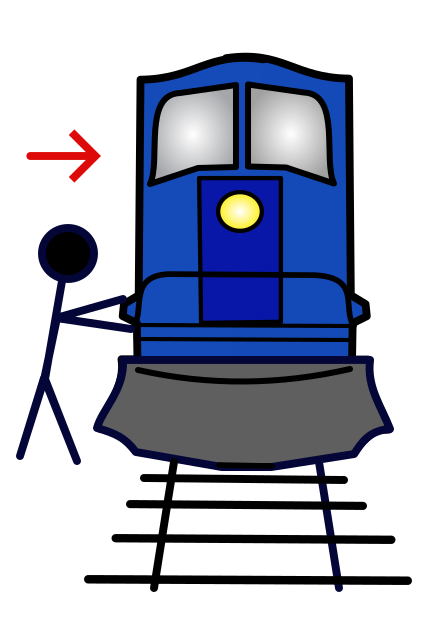
\includegraphics[width=0.8\textwidth]{train.png}


Now that you know about dot products: The work you do is the dot
product of the force vector you apply and the displacement vector of the train. (The displacement
vector is the vector that tells how the train moved while you pushed it.) \index{work}

Similarly, we mentioned that power is the product of the force you apply and the velocity of the
mass you are applying it to. It is actually the dot product of the force vector and the velocity vector.\index{power}

For example, if you are pushing a sled with a force of 10 newtons and it is moving 2 meters per second, 
but your push is 20 degrees off, you aren't transferring 20 watts of power to the sled.  
You are transferring $10 \times 2 \times \cos(20 \text{ degrees}) \approx 18.8$ watts of power.
%add ramps and sin

%FIXME combined chapter on dot product and cross product